\documentclass[conference]{IEEEtran}
\IEEEoverridecommandlockouts
% The preceding line is only needed to identify funding in the first footnote. If that is unneeded, please comment it out.
\usepackage{cite}
\usepackage{amsmath,amssymb,amsfonts}
\usepackage{algorithm}
\usepackage{algorithmic}
% \usepackage[noend]{algpseudocode} % http://ctan.org/pkg/Algorithmicx
\usepackage{graphicx}
\graphicspath{{figs/}}
\usepackage{lipsum}
\usepackage{textcomp}
\usepackage{xcolor}
\usepackage{listings}
\usepackage{color}
% \usepackage[font=footnotesize,labelfont=bf]{caption} 
% \captionsetup[table]{skip=10pt}
\usepackage{array}
\usepackage{standalone}
\usepackage{tikz}
% \usepackage{subcaption}
\usepackage{authblk}
\newcommand{\Algorithmicbreak}{\textbf{break}}
\newcommand{\BREAK}{\STATE \Algorithmicbreak}
\newcommand{\ignore}[1]{}
\definecolor{codegreen}{rgb}{0,0.6,0}
\definecolor{codegray}{rgb}{0.5,0.5,0.5}
\definecolor{codepurple}{rgb}{0.58,0,0.82}
\definecolor{backcolour}{rgb}{0.95,0.95,0.92}

\lstdefinestyle{mystyle}{
	backgroundcolor=\color{backcolour},   
	commentstyle=\color{codegreen},
	keywordstyle=\color{magenta},
	numberstyle=\tiny\color{codegray},
	stringstyle=\color{codepurple},
	basicstyle=\footnotesize,
	breakatwhitespace=false,
	breaklines=true,                 
	captionpos=b,                    
	keepspaces=true,                 
	numbers=left,                    
	numbersep=5pt,                  
	showspaces=false,                
	showstringspaces=false,
	showtabs=false,                  
	tabsize=2
}

\lstset{style=mystyle}

\lstset{emph={%  
		async%
	},emphstyle={\color{blue}\bfseries}%
}

\def\BibTeX{{\rm B\kern-.05em{\sc i\kern-.025em b}\kern-.08em
T\kern-.1667em\lower.7ex\hbox{E}\kern-.125emX}}

\let\OLDthebibliography\thebibliography
\renewcommand\thebibliography[1]{
	\OLDthebibliography{#1}
	\setlength{\parskip}{0pt}
	\setlength{\itemsep}{0pt plus 0.3ex}
}

\usepackage{hyperref}

\begin{document}

\title{ASGriDS: Asynchronous Smart-Grids Distributed Simulator}


\author[1]{Takai-Eddine Kennouche}
\author[2]{Florent Cadoux}
\author[1]{Nicolas Gast}
\author[3]{Beno\^{i}t Vinot}
\affil[1]{Univ. Grenoble Alpes, CNRS, Inria, Grenoble INP*, LIG, 38000 Grenoble, France}
\affil[ ]{\{takai-eddine.kennouche, nicolas.gast\}@univ-grenoble-alpes.fr}
\affil[2]{Univ. Grenoble Alpes, CNRS, Grenoble INP*, G2ELab, 38000 Grenoble, France}
\affil[ ]{florent.cadoux@grenoble-inp.fr}
\affil[3]{Roseau Technologies, 38240 Meylan, France}
\affil[ ]{benoit.vinot@roseautechnologies.com}

% \author[ ]{ \\ \\ }
% \affil[ ]{ }
% \affil[ ]{ }
% \affil[ ]{ }
% \affil[ ]{ }
% \affil[ ]{ }

\maketitle
\begin{abstract}
We present ASGriDS, an asynchronous Smart Grid simulation framework. ASGriDS is multi-domain, it simultaneously models the power network along with its physical loads/generators, controllers, and communication infrastructure. ASGriDS provides a unified workflow in a pythonic environment, to describe, run and control complex SmartGrid deployment scenarios. ASGriDS is an event-driven simulator that can run in either real-time or accelerated real-time. As it is modular and its components interact asynchronously, it can run either locally on a distributed infrastructure, also in hardware-in-the-loop setups, and on top of emulated/physical communication links.
In this paper, we present the design of our simulator and we demonstrate its use with a generation control problem on a low voltage network. We use ASGriDS to deploy a real-time controller based on optimal power flow, on top of TCP and UDP based communication network, under various packet loss conditions.
\end{abstract}

\begin{IEEEkeywords}
real-time simulation, asynchronous, co-simulation, distributed simulation, HIL, Smart Grid Communication
\end{IEEEkeywords}

\section{Introduction}
The Smart Grid is a cyber - physical energy system, where the physical processes of a power system are strongly integrated with a communication network infrastructure and a set of possibly complex controllers. This vision of the modern power grid is motivated by the new challenges that are currently raised by the need to massively integrate distributed renewable energy generators. In addition to that, the Smart Grid is expected to satisfy growing reliability and efficiency demands, due to the fast transition to electrical power in public transportation systems and the growing usage of electrical vehicles. 

The Smart Grid needs to solve a variety of reliability and efficiency challenges~\cite{moslehiReliabilityPerspectiveSmart2010}. In this context, Information and Communication Technologies (ICT) come into play as an enabler for more intelligence to manage a complex set of operational, monitoring and optimization constraints, and allow for innovative solutions and novel applications.
On the other hand, understanding the ICT infrastructure's performance limits, such as managing packet transmission delays, is crucial for safety and stability of the power grid and efficiency of control, monitoring and recovery of the network.

New techniques are needed to properly prototype, test and validate a modern Smart Grid. Traditional testing and domain-specific simulation techniques and software tools only allow for partial representation of the system; for instance, there exists many domain-specific tools for the simulation of either the physics of a power grid, or for the simulation of telecommunication networks, but none of these tools are capable of embracing the complexity of a Smart Grid. Such tools are simply not sufficient to trace the complex behavior of intertwined power and telecommunication networks: for this purpose, multi-domain frameworks must be developed.

% To approach the problem of multi-domain simulation, we use \emph{co-simulation}, a method that has already been used in the Smart Grid literature, see \emph{e.g.}~\cite{Gupta2017, steinbrinkSimulationBasedValidationSmart2017}. 
% Co-simulation relies on exploiting tools that perform simulations on different domains, for instance a power simulator and a communications network simulator, in an orchestrated manner that guarantees time synchronization and communication of relevant information between the various domains of simulation.
% Integration of co-simulation with Hardware-In-the-Loop (HIL) is also a possible approach, that is geared towards more accurate accounting of the real-time behavior of specific grid components. In a combination with a distributed co-simulation strategy, more complex aspects of the Smart Grid can be modeled and studied in a multi-domain setup.

ASGriDS is developed to provide a modular and generic simulation description environment, that relies on an event-driven architecture to model power network components, and an asynchronous communication module that is scalable and reliable. Our framework is capable of running both local and distributed simulations. The nodes are asynchronous in the sense that they don't rely on heavy explicit synchronization, but they rely instead on the fact that their execution is driven by local clocks that are globally synchronous enough. This choice of implementation allows for realistic modeling of a real asynchronous Smart Grid behavior. It is also technically required to be able to account for real-time execution and Hardware-In-the-Loop (HIL) integration.
In addition, our framework is capable of modeling complex communication network behavior, through the use of Linux network emulation that permits rich tuning capabilities of delay, jitter, loss, duplication, reordering, corruption and rate. This allows the modeling of wired and wireless networks~\cite{hemminger2005network}.

The rest of the paper is organized as follows. In Section~\ref{related_work}, we review the state of the art of Smart Grid simulators, and put that in contrast with our own proposal. We describe the architecture and design choices of ASGriDS in Section~\ref{design} and evaluate its performance in Section~\ref{perf}. Finally, we present in Section~\ref{case_study} a case study concerning photovoltaic production control, in a low voltage network and lossy communication.

\section{Related Work} \label{related_work}
%EPCOH + GECO
The Electric Power and Communication Synchronizing Simulator (EPOCH)~\cite{hopkinsonEPOCHSPlatformAgentbased2006}, is a simulation framework that aims to study complex scenarios involving combined power and communication networks. EPOCH runs in a federated simulation environment, using PSCAD and PSLF for power simulations and UC Berkeley’s Network Simulator 2 (NS-2)~\cite{NetworkSimulatorNs2} for communication network simulations, with fixed time-stepping clock synchronization.

The Global Event-Driven Co-Simulation Framework (GECO)~\cite{linGECOGlobalEventDriven} is another framework that targets power system monitoring and control using a communication network. 
It also combines PSLF power system simulator and NS-2, but differs than EPOCH in that it uses a global event-driven co-simulation environment. GECO ensures full synchronization of events, by encapsulating dynamic power system simulation runs in discrete events queued in a global events queue and ordered with the network simulator events.

Another co-simulation framework is the Integrated co-Simulation of Power and ICT systems for Real-time Evaluation (INSPIRE)~\cite{georgINSPIREIntegratedCosimulation2013}. INSPIRE co-simulation environment consists of running DIgSILENT PowerFactory for power simulation, in conjunction with OPNET Modeler with a model of IEC 61850 communication protocol. Both are orchestrated with dynamic time-stepped clock.

%GRIDSpice
% GridSpice~\cite{andersonGridSpiceDistributedSimulation2014} is cloud-based and synchronized distributed platform, that relies on using a global simulation time-stepping clock to synchronize worker nodes in a cluster environment. It integrates Gridlab-D for generation and Distribution and MATPOWER for optimal power flow based control. The focus of GridSpice being mainly power-oriented, although it seems well designed and maintained, it doesn't really model network communication, which we consider a serious drawback for Smart Grid studies.

% We can find in~\cite{SGsimCosimulationFramework}, and~\cite{o.troianoCosimulatorPowerCommunication2016}, other examples of co-simulation based on time synchronization driven by OMNET++ network simulator, with OpenDSS and power simulator, in a master-slave architecture. While in~\cite{kimCoSimulatingCommunicationNetworks2018}, the same tools are orchestrated under a global event-driven scheduler.
A different simulation approach is followed in MECSYCO~\cite{vaubourgMultiagentMultiModelSimulation2015}, where the authors adhere to strict formalism using a Discrete Event System Specification (DEVS) to describe their multi-agent system. The interaction of their systems, though, is always strictly synchronized and does not provide any real time capabilities or the possibility of interaction with components outside the simulator.

T-RECS~\cite{acharaTRECSVirtualCommissioning2018} is another interesting simulator, its stated objectives are close to what we intend to develop in ASGriDS, in that it incorporates network emulation for more realistic control over the communication medium, and provides an API for the interaction with pre-existing components. However, as pointed by their authors in~\cite{acharaTRECSVirtualCommissioning2018}, it cannot scale to more than ten or a few tens of nodes, whereas ASGriDS can scale to hundreds. 

%Table~\ref{rev_compare} summarizes the various simulators, using what 
%We believe that the key elements of a Smart Grid simulation tool are:  Power System Simulator, Communication Simulation, Time Strategy, %Scalability and real-time capability.
It is noticeable that a limiting factor for realism and scalability of simulation, is the constraints of strong event/time synchronization among simulation components, and/or the implementation of a global event scheduler. Time synchronization can be a very fit choice, if the goal is to model synchronous systems, and/or to guarantee reproducible simulations and easy testing/debugging of certain system's aspects, but it falls short to capture the nature of an actually asynchronous system: such a system may only be accurately modelled by means of an asynchronous simulation framework, without a compromise in terms of accuracy~\cite{ghoshRoleModelingAsynchronous2002}. 
On the other hand, a global event scheduler, does not allow for any real-time execution, and limit the possibility to interact with other real-time components of the system.

Our work is intended to provide scalability of simulation, realism of modeling and flexibility of scenario description, through an asynchronous design and event-driven node model.
\begin{itemize}
	\item \textbf{Asynchronism}: ASGriDS does not enforce explicit time synchronization of the different nodes. Each node is driven by its local system's clock. %In addition, the design that we adopted allows to control the timing API implementation provided to the nodes, thus we can easily convert the simulation to a global stepped simulated time if global synchronization is actually needed (\emph{e.g.} for debugging purposes).
	Asynchronous communication is also used to decouple network I/O operations from nodes internal operations.
	\item \textbf{Real-time}: The simulation nodes all run in real-time, in the sense that they are driven by system's real-time clock. This allows the nodes to interact with the outside world --- for example, with a real communication infrastructure.
	\item \textbf{Scalability}: Scalability comes as a consequence of the modularity, event-driven and asynchronism of our architecture, as we show in section \ref{perf}.
	The socket-based communication module, also permits scalability both locally and on a distributed deployment, without sacrificing of its key features of asynchronism and real-time execution.
\end{itemize}

Our framework provides the necessary architecture for complex modeling of power/communication interactions, using either emulation of the ICT network, simulation models or interaction with real setup.

% \begin{table*}[ht]
% 	\centering
% 	\def\arraystretch{1.5}%
% 	\begin{tabular}{|c|c|c|c|c|c|}
% 		\hline 
% 			& \shortstack{\\Power System \\ Simulator}  & \shortstack{Communication\\Simulation}  & \shortstack{Time\\Strategy} & Scalability & real-time \\ 
% 		\hline 
% 		EPOCHS\cite{hopkinsonEPOCHSPlatformAgentbased2006} & PSCAD, PSLF & NS-2 & Time Stepping & High & No \\ 
% 		\hline 
% 		INSPIRE\cite{INSPIREIntegratedCosimulation} & DIgSILENT & OPNET & \shortstack{Time Stepping}  & High & No \\ 
% 		\hline 
% 		GECO\cite{linGECOGlobalEventDriven} & PSLF & NS-2 & Global Events Queue & High & No \\ 
% 		\hline 
% %%% 	GRIDspice\cite{andersonGridSpiceDistributedSimulation2014} &  &  &  &  &  \\ 
% %%% 	\hline 
% %%%		%SGsim\cite{SGsimCosimulationFramework} &  &  &  &  &  \\ 
% %%%		%\hline 
% %%%		%MOSAIK\cite{schutteMosaikFrameworkModular2011} &  &  &  &  & No \\ 
% %%%		%\hline 
% %%%		VPNET\cite{liVPNETCosimulationFramework2011} & VTB & OPNET & Time Stepping & Limited & No \\ 
% %%%		\hline 
% %%%		%ADEVS\cite{nutaroIntegratedHybridSimulationElectric2007} &  &  &  &  &  &  \\ 
% %%%		%\hline 
% %%% 		Greenbench\cite{weiGreenbenchBenchmarkObserving2014} & PSCAD & OMNET++ & Global Events Queue & Limited & No \\ 
% %%% 		\hline 
% %%% 		PowerNet\cite{SmartGridCommunication} & Modelica & NS-2 & Time Stepping & Limited & No \\ 
% %%% 		\hline 
% %%%		%Hahn et. al.\cite{venkataramananreal-timeCosimulationTestbed2016} &  &  &  &  &  \\ 
% %%%		%\hline 
% 		T-RECS.\cite{acharaTRECSVirtualCommissioning2018} & Custom & Mininet Emulation & real-time & Limited & Yes \\ 
% 		\hline 
% 		MECSYCO\cite{vaubourgMultiagentMultiModelSimulation2015a} & Flexible & Flexible & Global Events Queue & High & No \\ 
% 		\hline 
% %%%		%PVInGrid\cite{bottaccioliPVInGridDistributedInfrastructure2017} &  &  &  &  &  \\ 
% %%%		%\hline 
% %%%		%Yang et. al.\cite{manbachireal-timeCoSimulationPlatform2016} &  &  &  &  &  \\
% %%%		%\hline 
% %%%		%Troiano et. al. \cite{o.troianoCosimulatorPowerCommunication2016} & & & & & \\
% %%%		%\hline
% %%%		%Hua et. al. \cite{linPowerSystemCommunication2011} & & & & & \\
% %%%		%\hline
% %%%		%Karnouskos et. al. \cite{karnouskosSimulationSmartGrid2009} & & & & & \\
% %%%		%\hline
% %%%		%Kim et. al. \cite{kimCoSimulatingCommunicationNetworks2018} & & & & & \\
% %%%		%\hline
% 		ASGriDS & \shortstack{flexible\\pandapower as example} & \shortstack{flexible\\netem as default emulation} & Event-Driven & High & Yes\\
% 		\hline
% 	\end{tabular}
% 	\caption{Comparison of some of the existing simulators integrating Smart Grid Communication}
% 	\label{rev_compare}
% \end{table*}

\section{Design of ASGriDS}\label{design}

The general overview of ASGriDS's architecture is outlined in Figure~\ref{sens_arch}. The components shown in the figure represent the different aspects of a Smart Grid, whether it is the power networks simulation, the optimization and control or the network communication. These components, as seen in the figure, interact with each other at two separate but complimentary planes, a \textbf{Deployment Plane} and a \textbf{Communication Plane}.
In this section, we describe these two operational planes of the simulator, after which we discuss the various building blocks of ASGriDS and how it integrates both network emulation for ICT modeling, and electrical network simulation.

\begin{figure}[htp]
	\centering%
	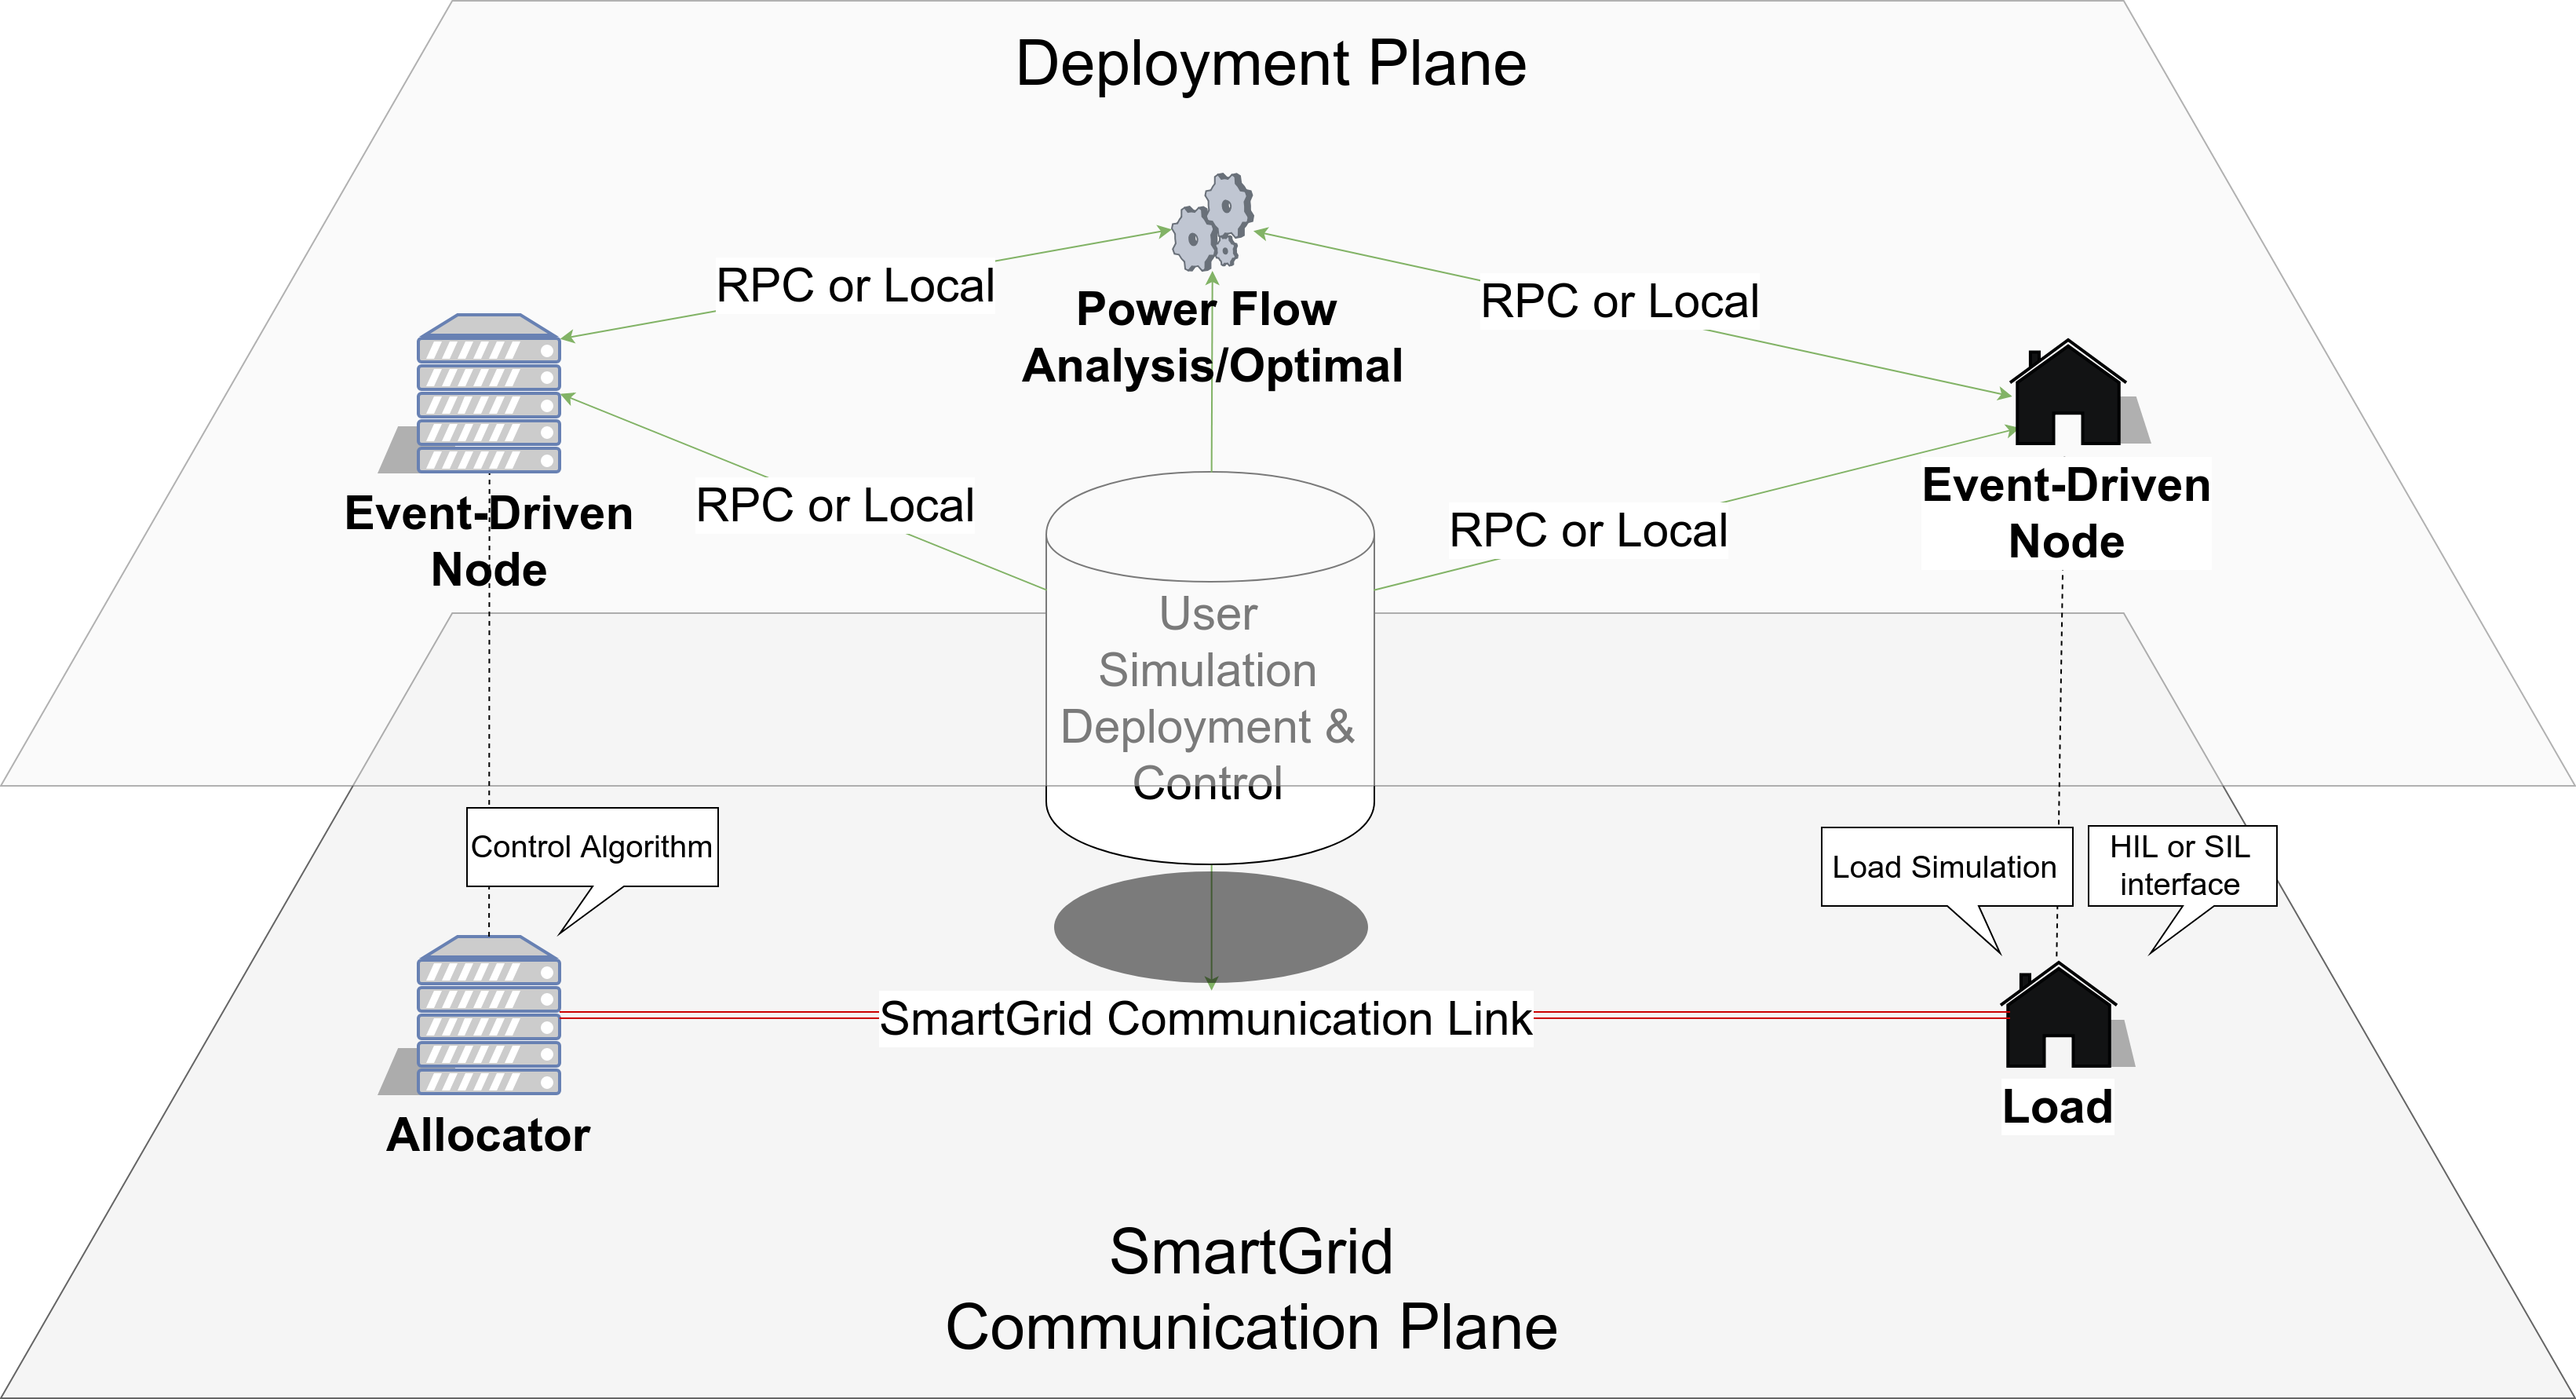
\includegraphics[width=0.5\textwidth]{sens_arch.png}%
	\caption{Simulation Deployment Architecture}%
	\label{sens_arch}%
\end{figure}

\subsection{Deployment Plane}

At the Deployment Plane level, ASGriDS deploys and orchestrates the simulation, the traffic flowing between the components at this level is exclusively the traffic necessary to control the various distributed elements of the simulator. The distinction between this and the actual simulation traffic is important, for instance in a distributed scenario one might want to change the behavior of a controller reployed remotely, or provide a remote node with a new production profile, or schedule some events, this will incur network traffic generated by the object-proxying mechanism that we rely on, this traffic isn't what we would like to observe or interact with, but it is necessary for simulation deployment. On a local scenario, this traffic will simply be the communication between system processes/threads.
ASGriDS basically triggers a ``remote object'' mode when run distributively that allows the user to handle simulation components, and network nodes as if they were running locally. This was possible using the concept of object-proxying and remote method invocation, and their implementation provided by the free and open-source library \texttt{RPyC}~\cite{RPyCTransparentSymmetric}. 
% Listing~\ref{rpyc_ex} is snippet code of who to automate remote node deployment/execution and remote object communication. We will described what a ``Node'' is in Section~\ref{rt_node}.

% % \begin{lstlisting}[language=python, caption=Creating remote nodes, label=rpyc_ex]
% % from plumbum import SshMachine
% % from rpyc.utils.zerodeploy import DeployedServer
% \begin{lstlisting}[language=python, caption=Creating remote nodes, label=rpyc_ex]
% remote_machine = SshMachine(hostname='hostname', 
%     username='username', password='password')
% remote_server = DeployedServer(remote_machine)
% conn = remote_server.classic_connect()
% Node = conn.modules['Node']
% node = Node()
% \end{lstlisting}

\subsection{Smart Grid Communication Plane}\label{sgcomm_plane}

At the Smart Grid Communication Plane level, ASGriDS simulates the actual communication network of interest for the end-users, where the traffic that is flowing is supposed to represent a real Smart Grid deployment traffic.
As we mentioned before, ASGriDS can be deployed on a variety of ICT models, whether emulated, simulated or real. By default, it allows very easy and flexible manipulation of the communication link between simulated nodes, through binding to a linux local network interface (local loop or virtual interface). Network impairments (delay, packet loss, duplication\dots) can then be controlled by the user through an interface to linux traffic shaping (\textit{tc})~\cite{hubert2002linux} utility and the \textit{netem} module~\cite{hemminger2005network}.


\subsection{Event-Driven Real-Time Node}\label{rt_node}

The basic component of the proposed framework is a real-time Event-Driven ``Node'', that is shown in Figure~\ref{async_comm}.
The ``Node'' component of ASGriDS, is an event-driven. It can be deployed as a process, a thread or a remote object in a distributed simulation. It interacts with its environment is callback-based, for instance when handling network events as in Figure~\ref{async_comm}. Most importantly, a node can be easily deployed to interact with any real-time source of events, such as hardware component (\emph{e.g.} real communication network) or software implementation of a certain behavior, that can already be available to the user through external libraries, either to test/validate software/hardware components or to implement new ones in a configuration as close to reality as possible. This renders the framework fit for a variety of HIL and Software-In-the-Loop (SIL) setups.

% \begin{figure}[htp]
% 	\centering%
% 	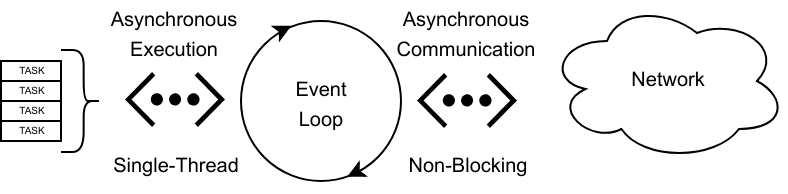
\includegraphics[width=0.4\textwidth]{event_driven_node.png}%
% 	\caption{Event-Driven Node}%
% 	\label{event_driven_node}%
% \end{figure}

%{\color{red}\lipsum[1-2]}

\subsection{Asynchronous Communication} \label{AsyncComm}

\begin{figure}[htp]
	\centering
	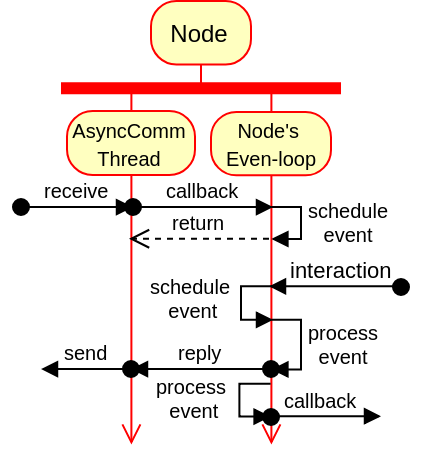
\includegraphics[width=.7\linewidth]{async_comm.png}
	\caption{Node --- Network interaction}
	\label{async_comm}
\end{figure}

In order for ASGriDS's ``Node'' to truly communicate in a network, it is supported by a communication layer module, and the interaction between the two happens through a callback mechanism, as shown in Figure~\ref{async_comm}.
In designing the module, our objective is a complete decoupling from the node through asynchronism and non-blocking network Input/Output operations, and pluggability in the sense that the communication layer can be modified/extended and easily plugged into a ``Node''.

We chose to implement this asynchronous communication (``AsyncComm'') module around \texttt{asyncio}~\cite{AsyncioAsynchronousPython}.
\texttt{asyncio} is a standard python library, it features flexible and industry-proven asynchronous API, and provides the necessary blocks to implement a communication layer that is completely asynchronous and modular, through its concurrent execution model and customizable event-loops.

% The ``AsyncComm'' module internally uses \texttt{ZeroMQ}'s ``DEALER'' and ``ROUTER'' sockets, handled in an \texttt{asyncio} ``context''. Listing~\ref{lst_zmq} shows the basic operation operation of creating said sockets. Basically, each node identifies its communicating peers using and identity and creates a ``DEALER socket'' for every peer-to-peer link. As a consequence, ASGriDS can run completely distributed, in either centralized or peer-to-peer topologies out of the box, to implement complex distributed applications in the domains of optimization and control.

% \begin{lstlisting}[language=python, caption=Creating remote nodes, label=lst_zmq]
% import zmq
% import asyncio
% import zmq.asyncio

% \begin{lstlisting}[language=python, caption=Creating remote nodes, label=lst_zmq]
% loop = asyncio.new_event_loop()
% asyncioset_event_loop(self.loop)
% context = zmq.asyncio.Context()
% poller = zmq.asyncio.Poller()
% server = context.socket(zmq.ROUTER)
% clients = {} # to define

% async def listen():
% 	while True:
% 		items = dict(await poller.poll(timeout))
% 		if server in items:
% 			identity, msg = await socket.recv_multipart()
% async def send(msg, dst):
% 	if dst not in clients:
% 		clients[dst] = context.socket(zmq.DEALER)
% 		clients[dst].connect(dst)
% 	await clients[dst].send_multipart([msg])
% \end{lstlisting}
	
% if if __name__ == "__main__":
% 	loop.run_until_complete(asyncio.ensure_future(listen(), loop=loop))

% \end{lstlisting}

\subsection{Electrical Simulation Integration}

In ASGriDS, electrical simulation is handled as a background service, controlled at the Deployment Plane, and interfacing with various other simulation components at the Smart Grid Communication Plane. For instance, this service keeps track of the electrical network state by solving load flow equations in real time. It provides an interface to other nodes so that they can access their local electrical state (\emph{i.e.} voltage).

In our experiments (that we present in Section~\ref{perf} and~\ref{sec:case_study}), we implement this component around \texttt{pandapower}, a free and open-source python library that provides access to various power system simulations such as load flow and optimal power flow solvers. 

\section{Performance of ASGriDS}\label{perf}

In this section, we study the scalability of ASGriDS in terms of CPU and memory consumption. Our assumption is that for low-voltage distribution networks and micro-grids, a scalable simulator should be able to handle in the order of hundreds of network nodes. For an entire distribution network, one to two additional orders of magnitude may be necessary. 

To measure the scalability of ASGriDS, we design a set of experiments according to the architecture in Figure~\ref{sens_arch}. Every component of the simulation is run as an independent computation node, that is either part of the simulated grid (Smart Grid Communication Plane), \emph{i.e.} a load or a generator (PV or otherwise) or part of the simulation management (Deployment Plane). At the simulation plane, each node simulates either a network load or a PV generator. These nodes communicate with a special node acting as a central allocator as follows: each node reports its voltage measurements and current production/consumption levels, and receives production setpoints in the case if PV generators. The allocator is running a control algorithm, that observes the network state through the voltage measures and acts accordingly to keep the network stable within a defined voltage limit.

\subsection{System Resources Consumption}

We define a set of benchmarks by using \texttt{pandapower}'s implementation of Washington Case300 network as a base-case. By default this network includes 193 loads (which corresponds to 193 nodes in our simulator). To vary the number of nodes of the network, we add or remove randomly nodes of this network. Every simulated node will be generating fake producation/consumption values in the electrical network, these values will be reported to an allocator (controller) along with voltage measurements gathered from \texttt{pandapower}'s power flow analysis, the allocator will then \texttt{pandapower}'s optimal power flow solver to generate new setpoints for the nodes. 

\begin{figure}[htp]
	\centering%
	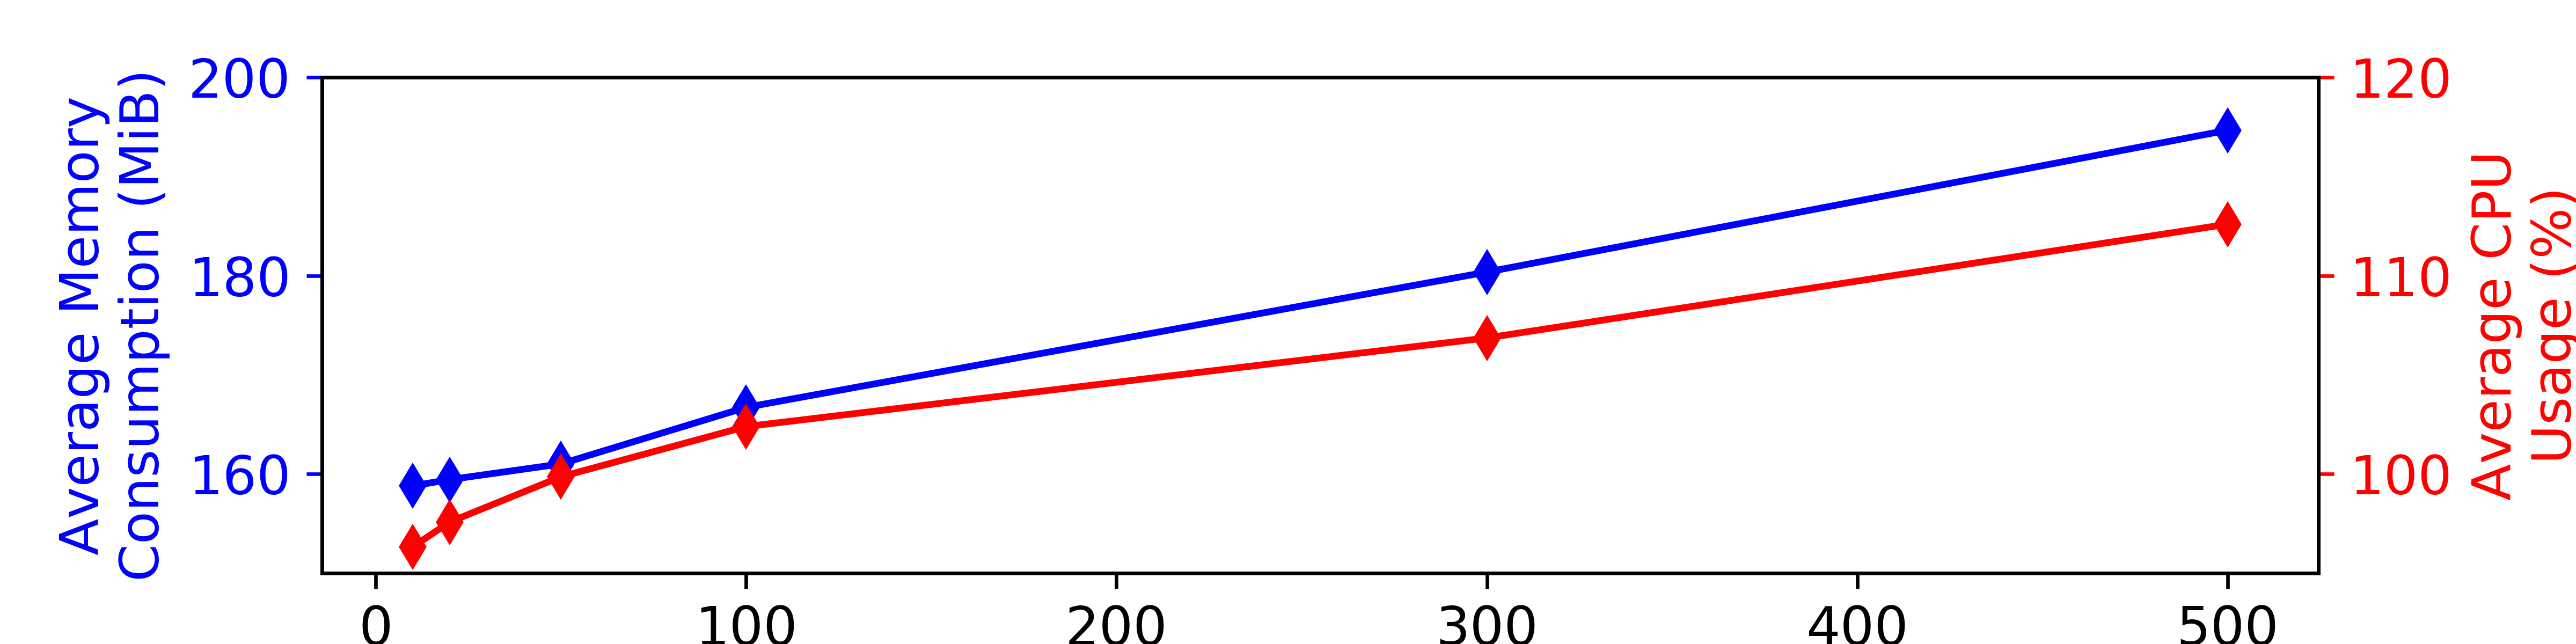
\includegraphics[width=1\linewidth]{mem_cpu.png}%
	\caption{ASGriDS's CPU and Memory consumption for various network sizes}%
	\label{sim_mem}
\end{figure}

In Figure~\ref{sim_mem}, we report the maximal memory usage of our simulator during the first 3 minutes of simulation as a function of of the number of nodes deployed.  We observe that the memory consumption remains limited and roughly equals $140$~MB plus $50$~kB per simulated node. Note that we also run the tests with other scenarios than the Washington Case300 and obtain similar values. 

In all of our experiments, the CPU usage for our simulator is mainly dominated by the load flow\ignore{solver that runs in an asynchronous while true loop (in order to be maintained up to date)}. To verify that \texttt{pandapower} was fit for the need of our simulator, we measured the time taken by this library to solve load flow and optimal power flow equations. Our measures show that solving one load flow takes less than $100$~ms while computing an optimal power flow takes a delay between $0.5$~s for small networks, and $2.5$~s for $\sim$200 nodes network.

% \begin{figure}[htp]
% 	\centering
% 	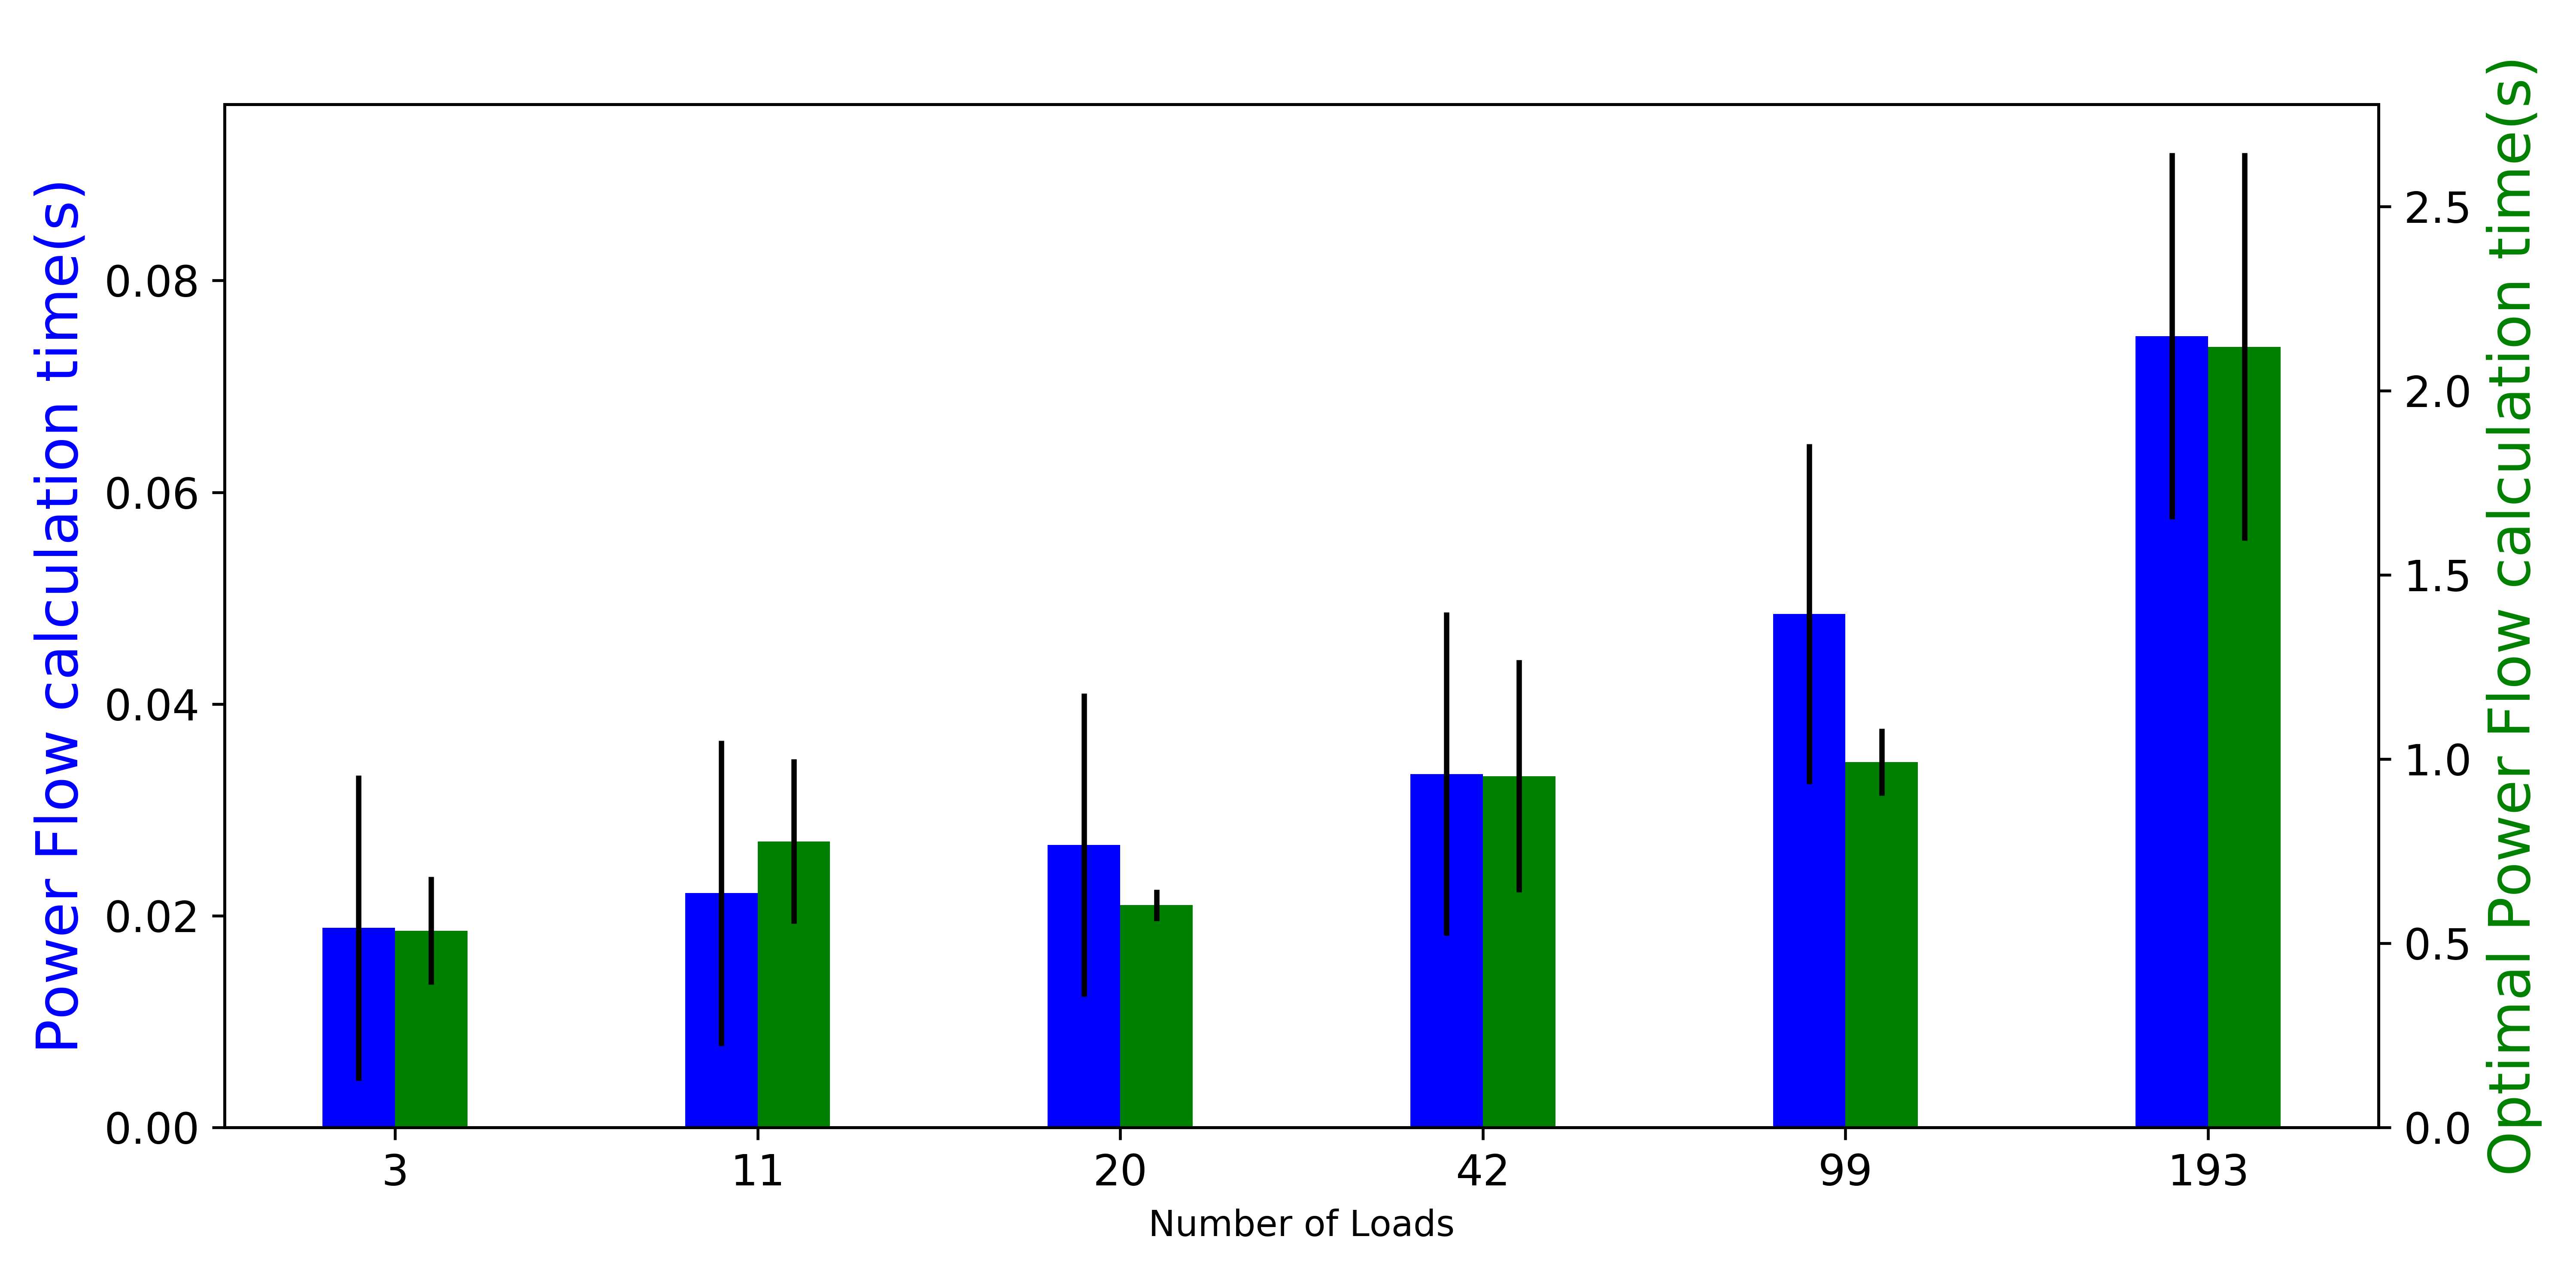
\includegraphics[width=\linewidth]{op_pp_time.png}
% 	\caption{Computation time of load flow and optimal power flow analysis by \texttt{pandapower}. Each bar corresponds to one example provided by \texttt{pandapower}.}
% 	\label{pp_time}
% \end{figure}

%\subsection{Case Study}
% \begin{figure}[b]
%   \centering
%   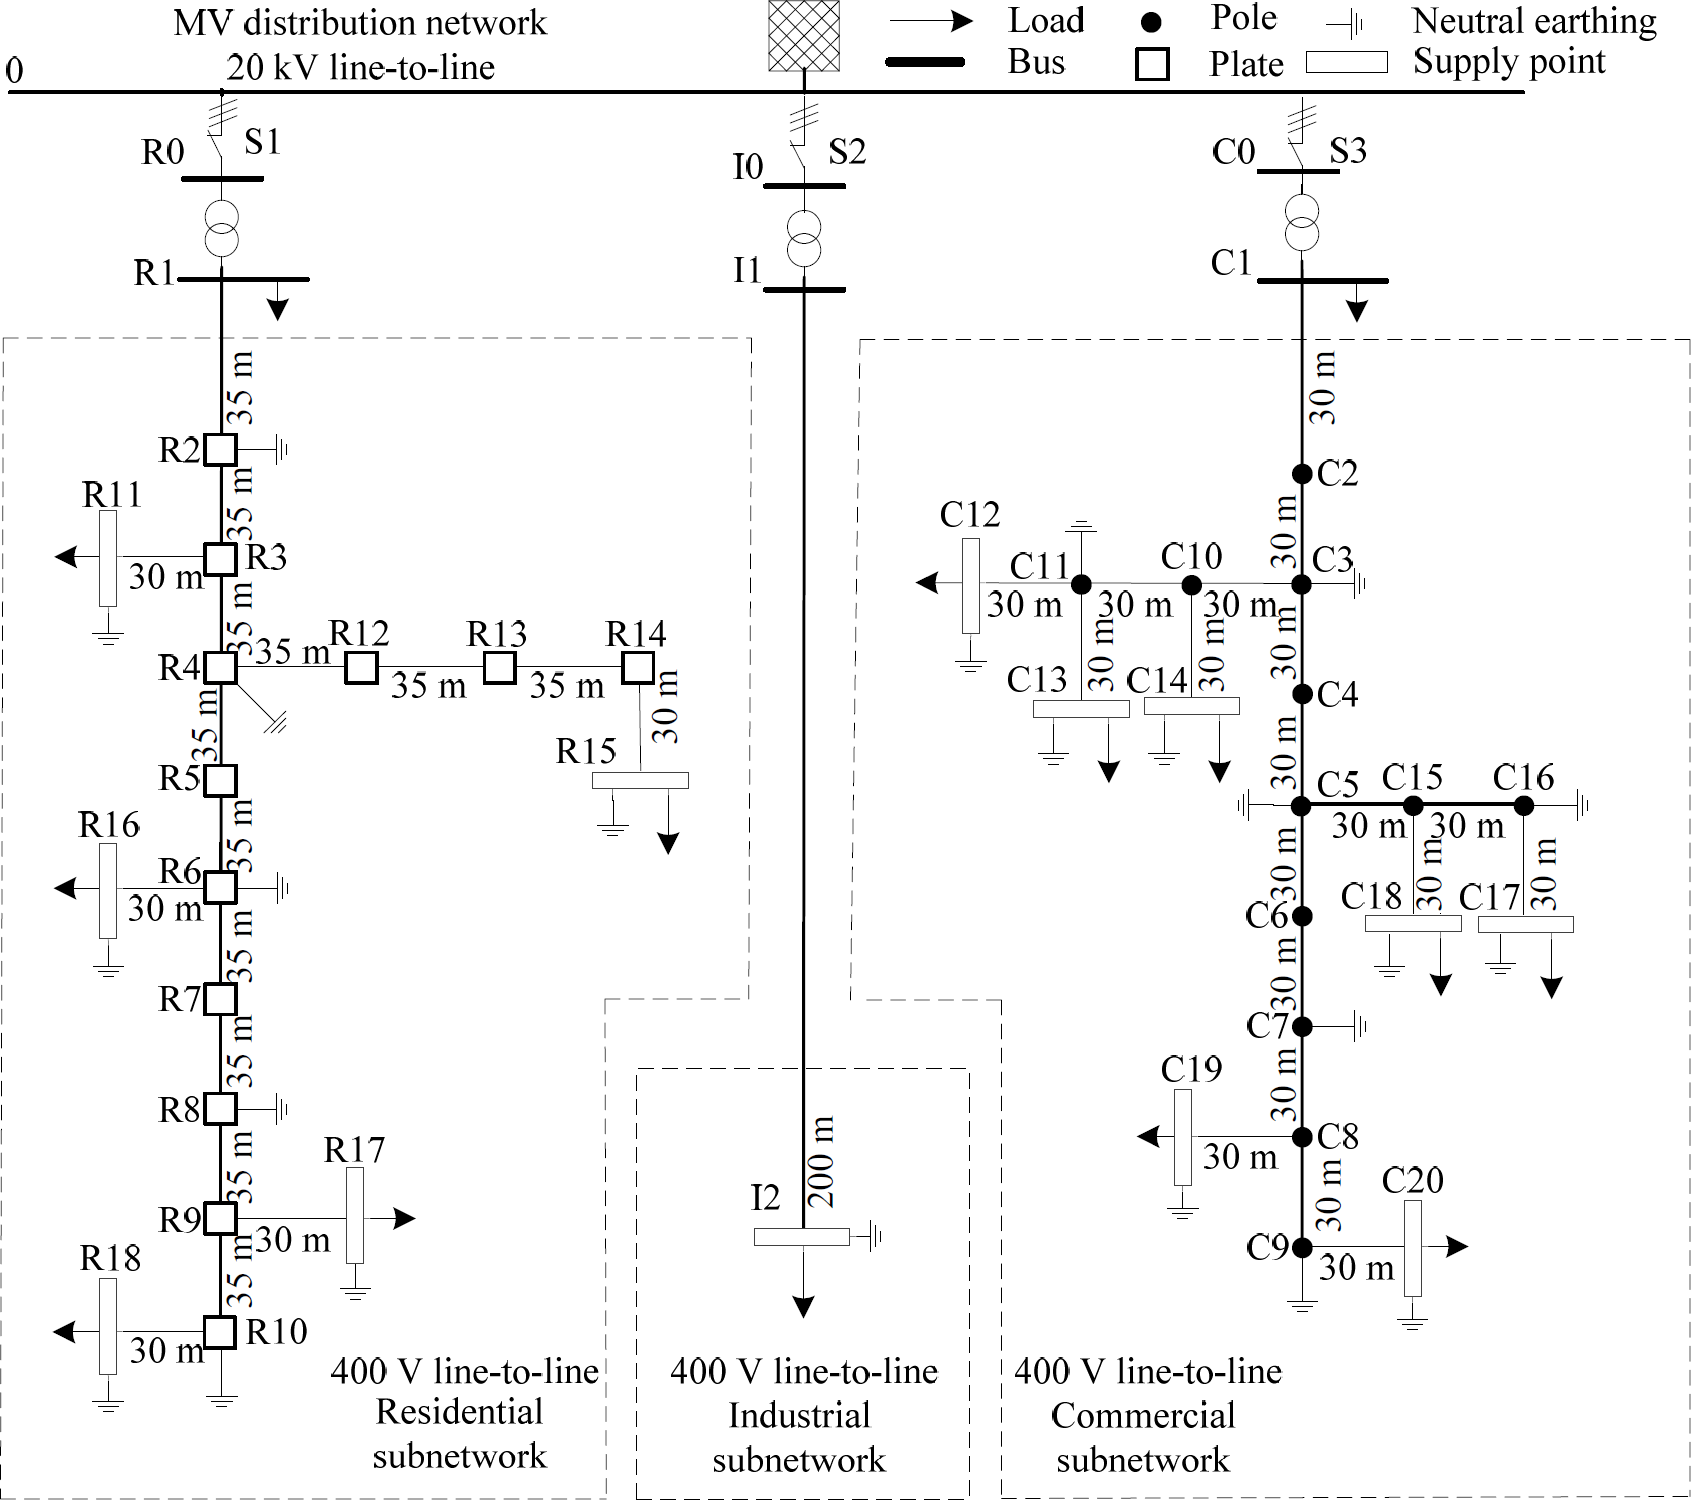
\includegraphics[width=0.5\textwidth]{cigre_network_lv.png}
%   \caption{The CIGRE low voltage distribution network that we use.}
%   \label{cigre_lv}
% \end{figure}

\section{Case Study: OPF-based Controller on a Lossy Network}\label{case_study}
\label{sec:case_study}


To demonstrate the capabilities of ASGriDS, we present a case study where we deploy CIGRE's low voltage network~\cite{BenchmarkSystemsNetwork2011}\ignore{ depicted in Figure~\ref{cigre_lv}} in ASGriDS. CIGRE's loads become "Nodes" capable of PV power generation, by incorporating load and production profiles from \cite{espinosa2015dissemination}. The low voltage network consists of 37 nodes distributed over residential, industrial and commercial sub-networks, and includes 6 residential loads, 8 commercial and one industrial. This benchmark encapsulates the most relevant technical aspects of a real electrical grid, and it is developed for the purpose of modeling and simulating modern micro-grids efficiently~\cite{papathanassiouBENCHMARKLOWVOLTAGE}.

In the deployed simulations, every load from the CIGRE network corresponds to a "Node" in ASGriDS, running 24h recorded consumption and PV production profiles from~\cite{espinosa2015dissemination}, read from a database. In the simulations, for practical reasons, we simulate the systems in accelerated real time (x300) so that 24h simulated time corresponds to 5min realtime. 

An allocator (controller) ``node'' runs the control loop as described in the petri net\cite{petersonPetriNets1977} diagram in Figure~\ref{pp_pi} and submits new PV production setpoints to all concerned nodes every cycle (15min simulation, 3s accelerated realtime). A power flow solver runs in the background (using \texttt{pandapower}) to provide timely voltage measurements to nodes (Deployment Plane). Each node reports this voltage value along with its consumption/production, to the allocator (Communication Plane). When a node receives a new setpoint, it implements the maximum between the new setpoint and the current maximum production capacity.

% \begin{algorithm}
% \algsetup{linenosize=\tiny}
% \small %\small, \footnotesize, \scriptsize, or \tiny
% \caption{Control loop with OPF}\label{alg_control}
% \begin{algorithmic}
%  \algsetup{linenosize=\tiny}
% \ENSURE $duty\_cycle \geqslant 0$
% \ENSURE $\|V\| \geqslant 0$ \COMMENT {Voltage values for all buses}
% \ENSURE $v_{max}$ \COMMENT {Bus voltage threshold}
% \WHILE{True}
% \STATE $optimize \leftarrow False$
% \STATE $sleep(duty\_cycle)$
% \FOR{$i=0$ to $\|V\|$}
% \IF{$V[i]~\geq~v_{\max}$}
% \STATE $optimize$ = True
% \BREAK
% \ENDIF
% \ENDFOR
% \IF{$optimize$}
% \STATE $A \leftarrow solve\_opf()$ \COMMENT{New generation setpoints}
% \FOR{$i=0$ to $\|A\|$}
% \STATE $submit(A(i))$
% \ENDFOR
% \ENDIF
% \ENDWHILE
% \end{algorithmic}
% \end{algorithm}


% \begin{algorithm}
% \algsetup{linenosize=\tiny}
% \small %\small, \footnotesize, \scriptsize, or \tiny
% \caption{Handling PV setpoints}\label{alg_alloc}
% \begin{algorithmic}
%     \ENSURE $max\_setpoint$
%     \STATE \textbf{Function} handle\_setpoint($setpoint$)
%     \IF{$allocation~\leq~max\_setpoint$}
%     \STATE $max\_setpoint = setpoint$
%     \ENDIF
%     \STATE \textbf{EndFunction}
% \end{algorithmic}
% \end{algorithm}



\begin{figure}[htp]
	\centering
	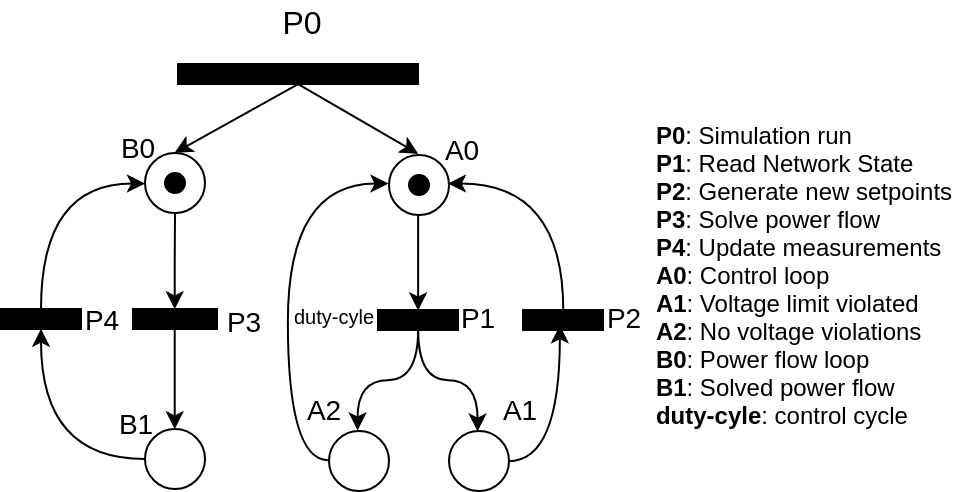
\includegraphics[width=\linewidth]{figs/pandapower.png}
	\caption{Power flow analysis and production control, running in parallel}
	\label{pp_pi}
\end{figure}

We use the experiments to observe the performance of an Optimal Power Flow based controller described in section \ref{opf_controller}. The controllers will be operating with a communication packet loss ranging between no loss (ideal communication), and $60~\%$ of packet loss (extreme conditions). The network is deployed on an emulated link, and losses are controlled through linux's \emph{netem} module. Recall that the network losses affect the transmission between the allocator node and the loads. The communication between the nodes and the power flow analyzer is not affected by the losses as such communications are done through the deployment plane.

% \begin{figure}[ht]
% 	\centering
% 	\includegraphics[width=.4\textwidth]{opp_time.png}
% 	\caption{Optimal power flow runtime for various network sizes}
% 	\label{opp_time}
% \end{figure}

% \subsection{PI Controller}
% \label{pi_controller}

% The simplest controller that we choose to implement is a basic PI controller. At a given time $t$, this controller measures an error $e(t)$ that is the maximum voltage on all bus minus the maximum admissible voltage $v_{\max}=1.05~p.u$. It uses this value to update an integrated error $I(t)$. Based on these values, the controller calculates a scaling factor $u\in[0,1]$. The control output $u$ is then send to all PV producers and acts as a quota: A PV producer that has a nominal capacity of $P_{\max}$ will be allowed to produce at most $u P_{\max}$. It will produce less if there is low irradiation. 

% The PI controller is summarized in the equation below: 
% \begin{equation}\label{pi_control}
% \begin{split}
% 	\text{Gather from all }  e(t) &:= v_{\max} - \max_{b\in\text{buses}}\{v_b(t)\}\\
% 	\text{Update } I(t) &:= I(t-1) + e(t) \Delta t\\
% 	\text{Send to all } u(t) &:= \max(0, \min( 1,  1 + \sigma \, e(t) + \tau \, I(t) )\\
% \end{split}
% \end{equation}
% In our experiments, the nominal power of all PV producer is $P_{\max}=30$~kW. $v_{\max}$ is the maximum allowed bus voltage, set to $1.05$~p.u. $\sigma$ and $\tau$ are the PI control parameters, set to $\sigma=5\times10^{-2}$~V$^{-1}$ and $\tau=4\times10^{-5}$~(Vs)$^{-1}$. The control is updated every $15$ min and $\delta t$ is the duration of a time step ($15$min=$900$s). 

\subsection{Optimal Power Flow Controller}\label{opf_controller}

We implement the Optimal Power Flow (OPF) control loop around the OPF formulation in Equation~\eqref{eq_opf_1}. Where $P$ is the production capacity every PV producer.
\begin{equation}\label{eq_opf_1}
\begin{split}
	\max & \sum_{i \in \text{PV generators}}{P_i} \\
	\text{subject to } 
	& V_{\min} \leqslant V_{g,i}  \leqslant V_{\max}, j\in\text{bus} \\
	& L_{k} \leqslant L_{\max,k}, k\in\text{transformer} \\
	& L_{l} \leqslant L_{\max,l}, l\in\text{line}\\
	& P_i \leqslant P_{i,\mathrm{max}}
\end{split}
\end{equation}
In our experiments, we use \texttt{pandapower} to solve the OPF (with default parameters). 
The constraints are 100~\% loading for branch elements, and $\pm$5\%~p.u. around nominal voltage for bus voltages. The value of $P_{i,\text{max}}$ is a forecast of what we think could be the maximal production of the PV panel $i$.
% \begin{equation}\label{eq_opf_2}
% 	\begin{split}
% 	& V_{\min,j} \leqslant V_{g,i}  \leqslant V_{\min,i}, j\in\text{bus} \\
% 	& L_{k} \leqslant L_{\max,k}, k\in\text{transfo} \\
% 	& L_{l} \leqslant L_{\max,l}, l\in\text{line}
% 	\end{split}
% \end{equation}


% \begin{figure}[ht]
% 	\centering
% 	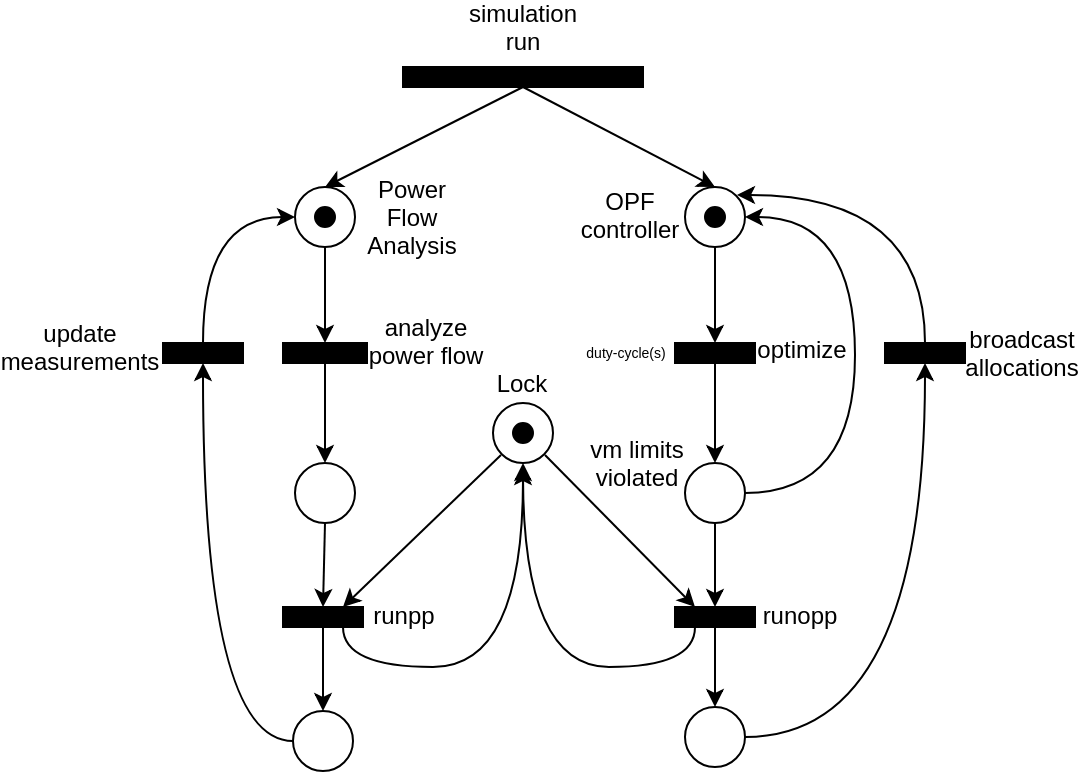
\includegraphics[width=.4\textwidth]{pp_opp.png}
% 	\caption{Petri Net for power flow analysis and Optimal Power Flow based control, with pandapower}
% 	\label{pp_opp}
% \end{figure}


% \begin{figure*}[ht]
% 	\begin{subfigure}{.5\textwidth}
% 		\centering
% 		\includegraphics[width=1\textwidth]{{figs/pi_load_127.0.0.1:5578}.png}
% 		\caption{Profile for load C12 (PI Controller)}
% 		\label{prod_c12_pi}
% 	\end{subfigure}%
% 	\begin{subfigure}{.5\textwidth}
% 		\centering
% 		\includegraphics[width=1\textwidth]{{figs/opf_load_127.0.0.1:5578}.png}
% 		\caption{Profile for load C12 (OPF Controller)}
% 		\label{prod_c12_opf}
% 	\end{subfigure}%
% 	\newline
% 	\begin{subfigure}{.5\textwidth}
% 		\centering
% 		\includegraphics[width=1\textwidth]{{figs/pi_bus_35}.png}
% 		\caption{Voltage for bus C12 (PI Controller)}
% 		\label{volt_c12_pi}
% 	\end{subfigure}%
% 	\begin{subfigure}{.5\textwidth}
% 		\centering
% 		\includegraphics[width=1\textwidth]{{figs/opf_bus_35}.png}
% 		\caption{Voltage for bus C12 (OPF Controller)}
% 		\label{volt_c12_opf}
% 	\end{subfigure}%
% 	\caption{CIGRE: Voltage and Load values}
% 	\label{cigre_values}
%   \end{figure*}
  

% \begin{figure}[ht]
% 	\begin{subfigure}{0.25\textwidth}
% 		\centering
% 		\includegraphics[width=1\textwidth]{{figs/ecdf_0loss}.png}
% 		\caption{Control with 0~\% packet loss}
% 		\label{prod_c12_pi}
% 	\end{subfigure}%
% 	\begin{subfigure}{.25\textwidth}
% 		\centering
% 		\includegraphics[width=1\textwidth]{{figs/ecdf_5loss}.png}
% 		\caption{Control with 5~\% packet loss}
% 		\label{prod_c12_opf}
% 	\end{subfigure}%
% 	\newline
% 	\begin{subfigure}{.25\textwidth}
% 		\centering
% 		\includegraphics[width=1\textwidth]{{figs/ecdf_15loss}.png}
% 		\caption{Control with 10~\% packet loss}
% 		\label{volt_c12_pi}
% 	\end{subfigure}%
% 	\begin{subfigure}{.25\textwidth}
% 		\centering
% 		\includegraphics[width=1\textwidth]{{figs/ecdf_20loss}.png}
% 		\caption{Control with 20~\% packet loss}
% 		\label{volt_c12_opf}
% 	\end{subfigure}%
% 	\caption{ECDF of {vm\_pu} values with different packet loss values}
% 	\label{sim_ecdf}
%   \end{figure}

\subsection{Numerical Results}

% In Figure~\ref{ecdf_loss} we show an Empirical Cumulative Distribution Function (ECDF) of all the voltage values at all buses. 
% We compare a situation with no loss (all control messages are received) and a very lossy network. 
% We observe that with zero packet loss, the optimal power flow manages to suppress most of the over-voltage events. 
% Note that even if this particularly favorable case, the optimal power flow does not suppress all over-voltage events because its only updates its decisions every 15 minutes. 
% When 60\% of the control packets are lost, the controller's performance is obviously worse. 

% \begin{figure}[ht]
% 	\centering%
% 	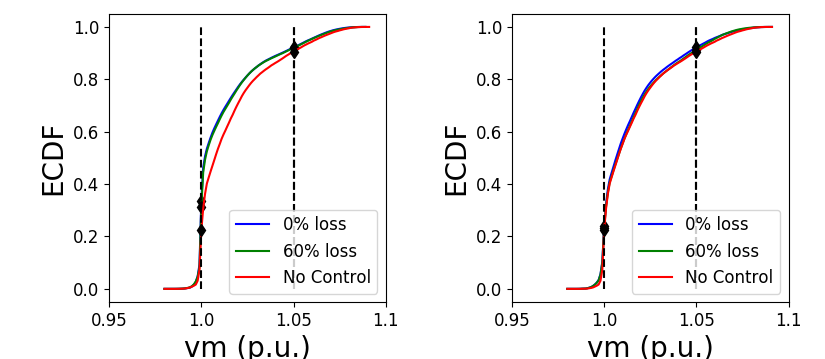
\includegraphics[width=0.5\textwidth]{figs/ecdf_loss.png}%
% 	\caption{OPF(left) vs PI(right) vs No Control, with packet loss}%
% 	\label{ecdf_loss}
% \end{figure}


In Figure~\ref{bars_loss} we plot the performance of the OPF controller, in terms of the rate of voltage violations (voltage outside 5\% of nominal value) detected from all measurements in the network, as a function of various losses configure in the communication channel, while using either TCP or UDP as a transport protocol.
The baseline (in red), is when there is no control. We observe that the OPF in TCP mode consistently outperforms the OPF in UDP mode, although the difference is small for packet loss of 0\%, 10\%, 20\% and 30\% the performance is very good in both cases. With 60\% packet loss, we notice that the controller manages to perform better with UDP, we explain that by the fact that TCP might exhibit high retransmission rate with such high packet loss, thus delivers outdated measurements and control information, the effect that is absent in UDP.
% In Figure~\ref{bars_power_loss} we can see another way of looking at the performance, eventhough TCP performs slightly better than UDP for most emulated packet losses, one could still favor UDP given that it results in less production loss, throughout the network (out of maximum 35.970 mW with no control).

\begin{figure}[ht]
	\centering
	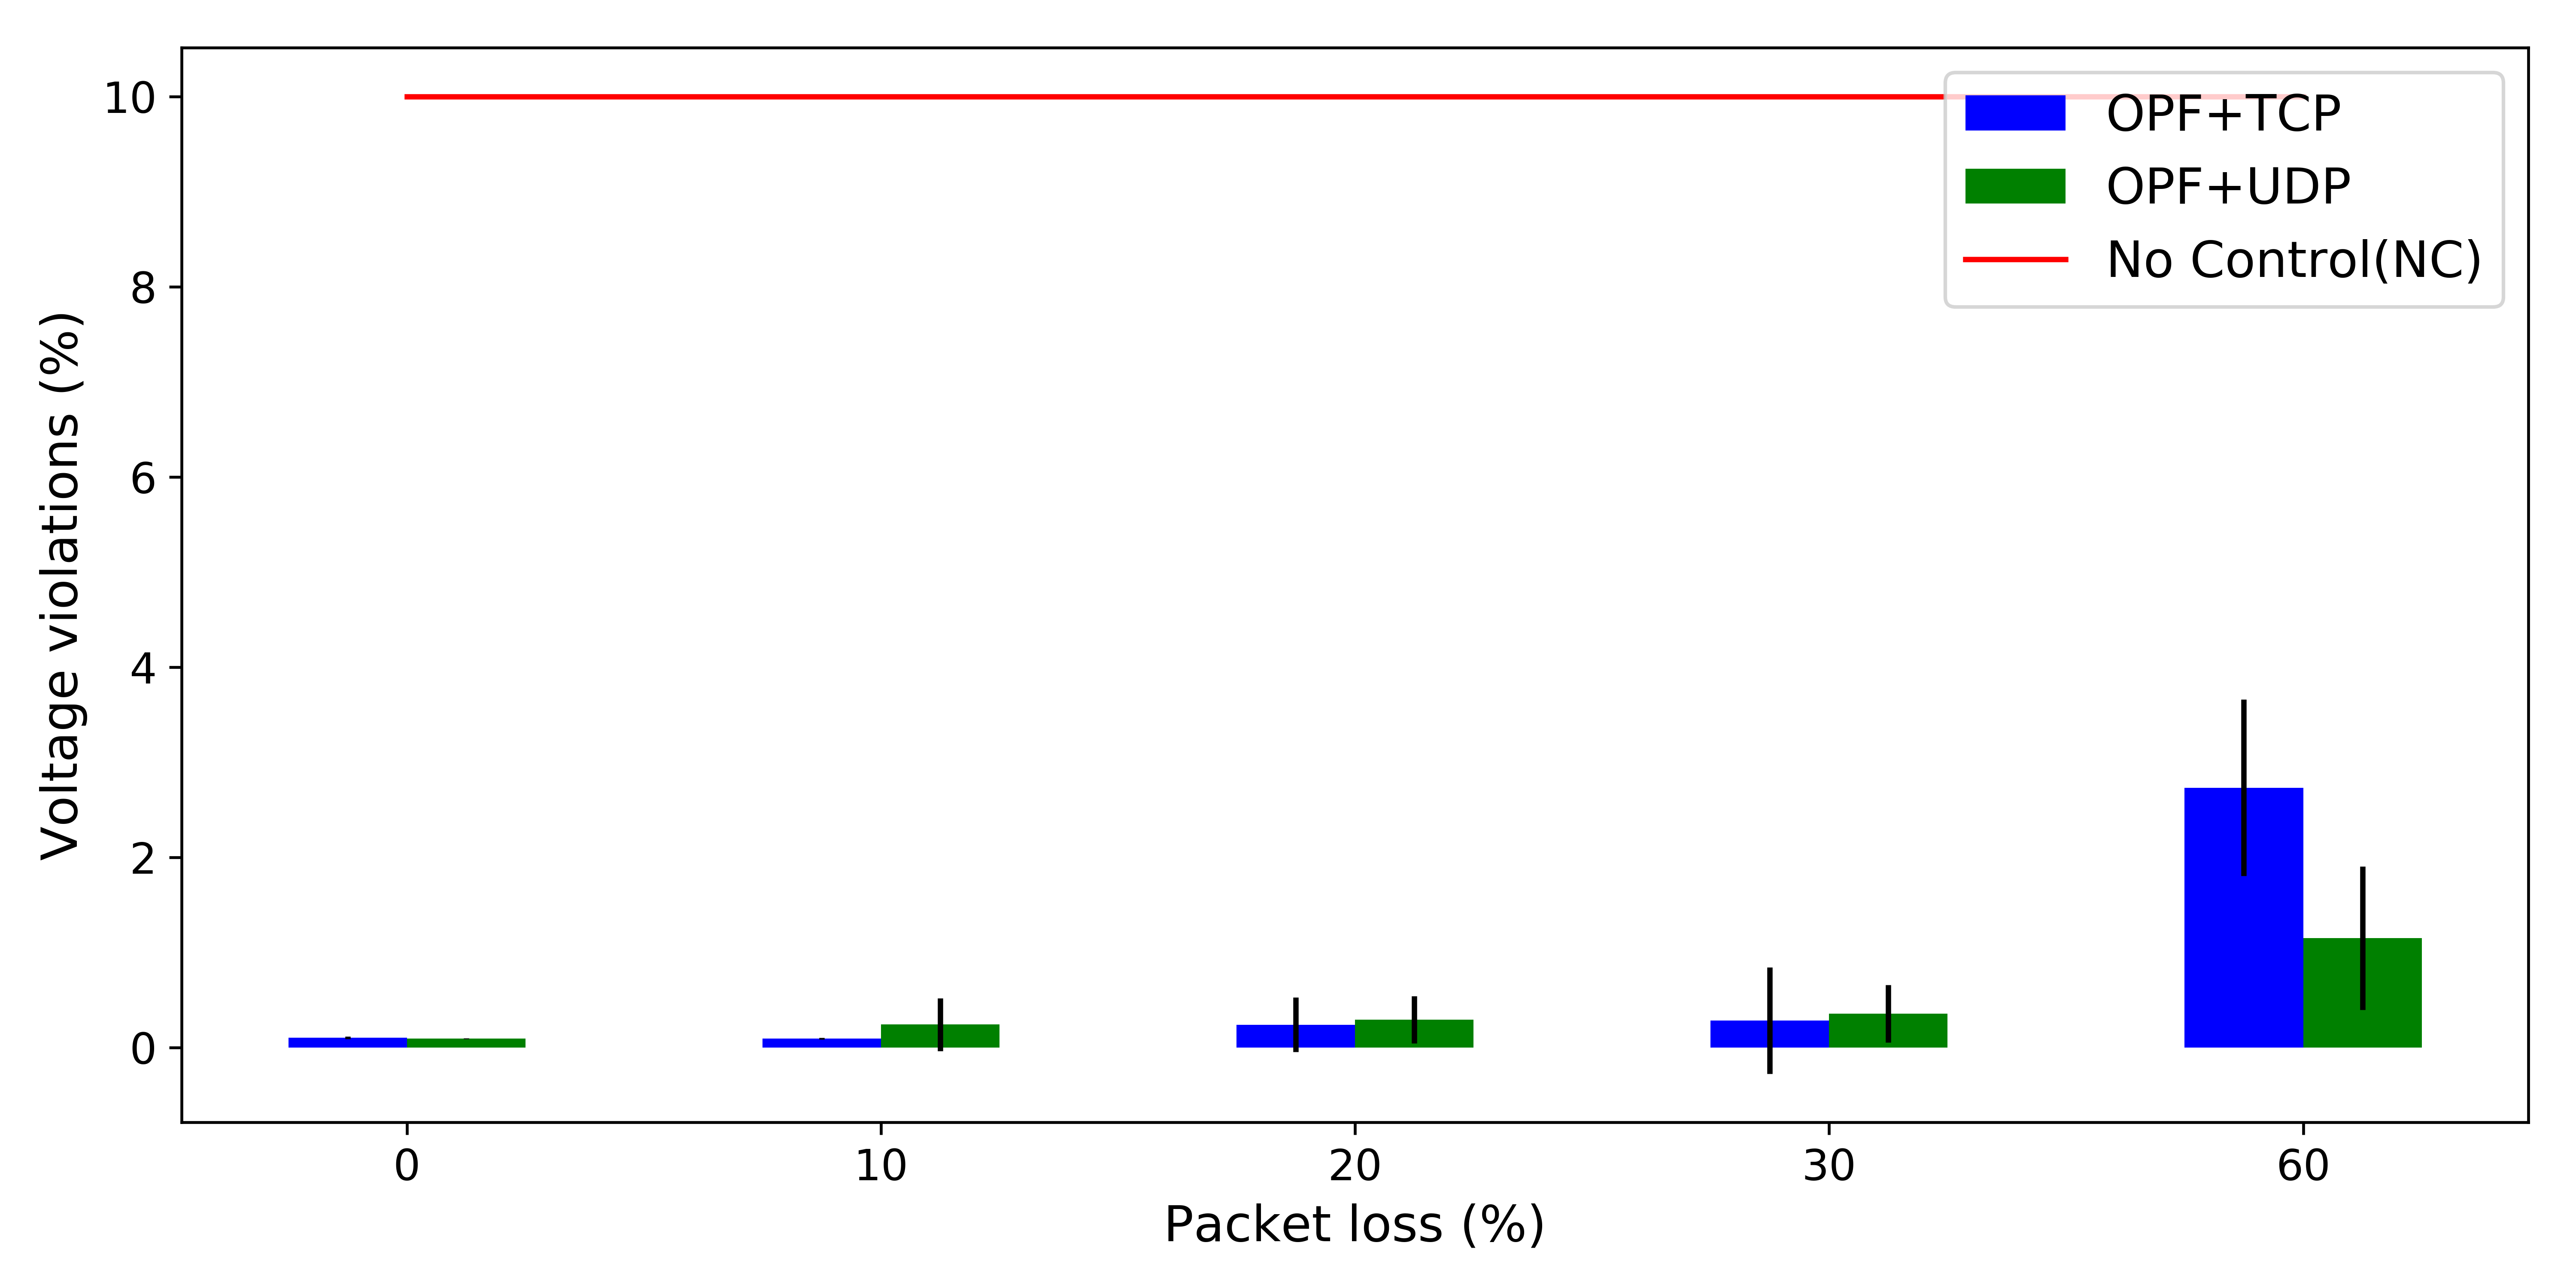
\includegraphics[width=0.5\textwidth]{bars_loss.png}
	\caption{Voltage violations with TCP/UDP communication on a lossy network}
	\label{bars_loss}
\end{figure}

% \begin{figure}[ht]
% 	\centering
% 	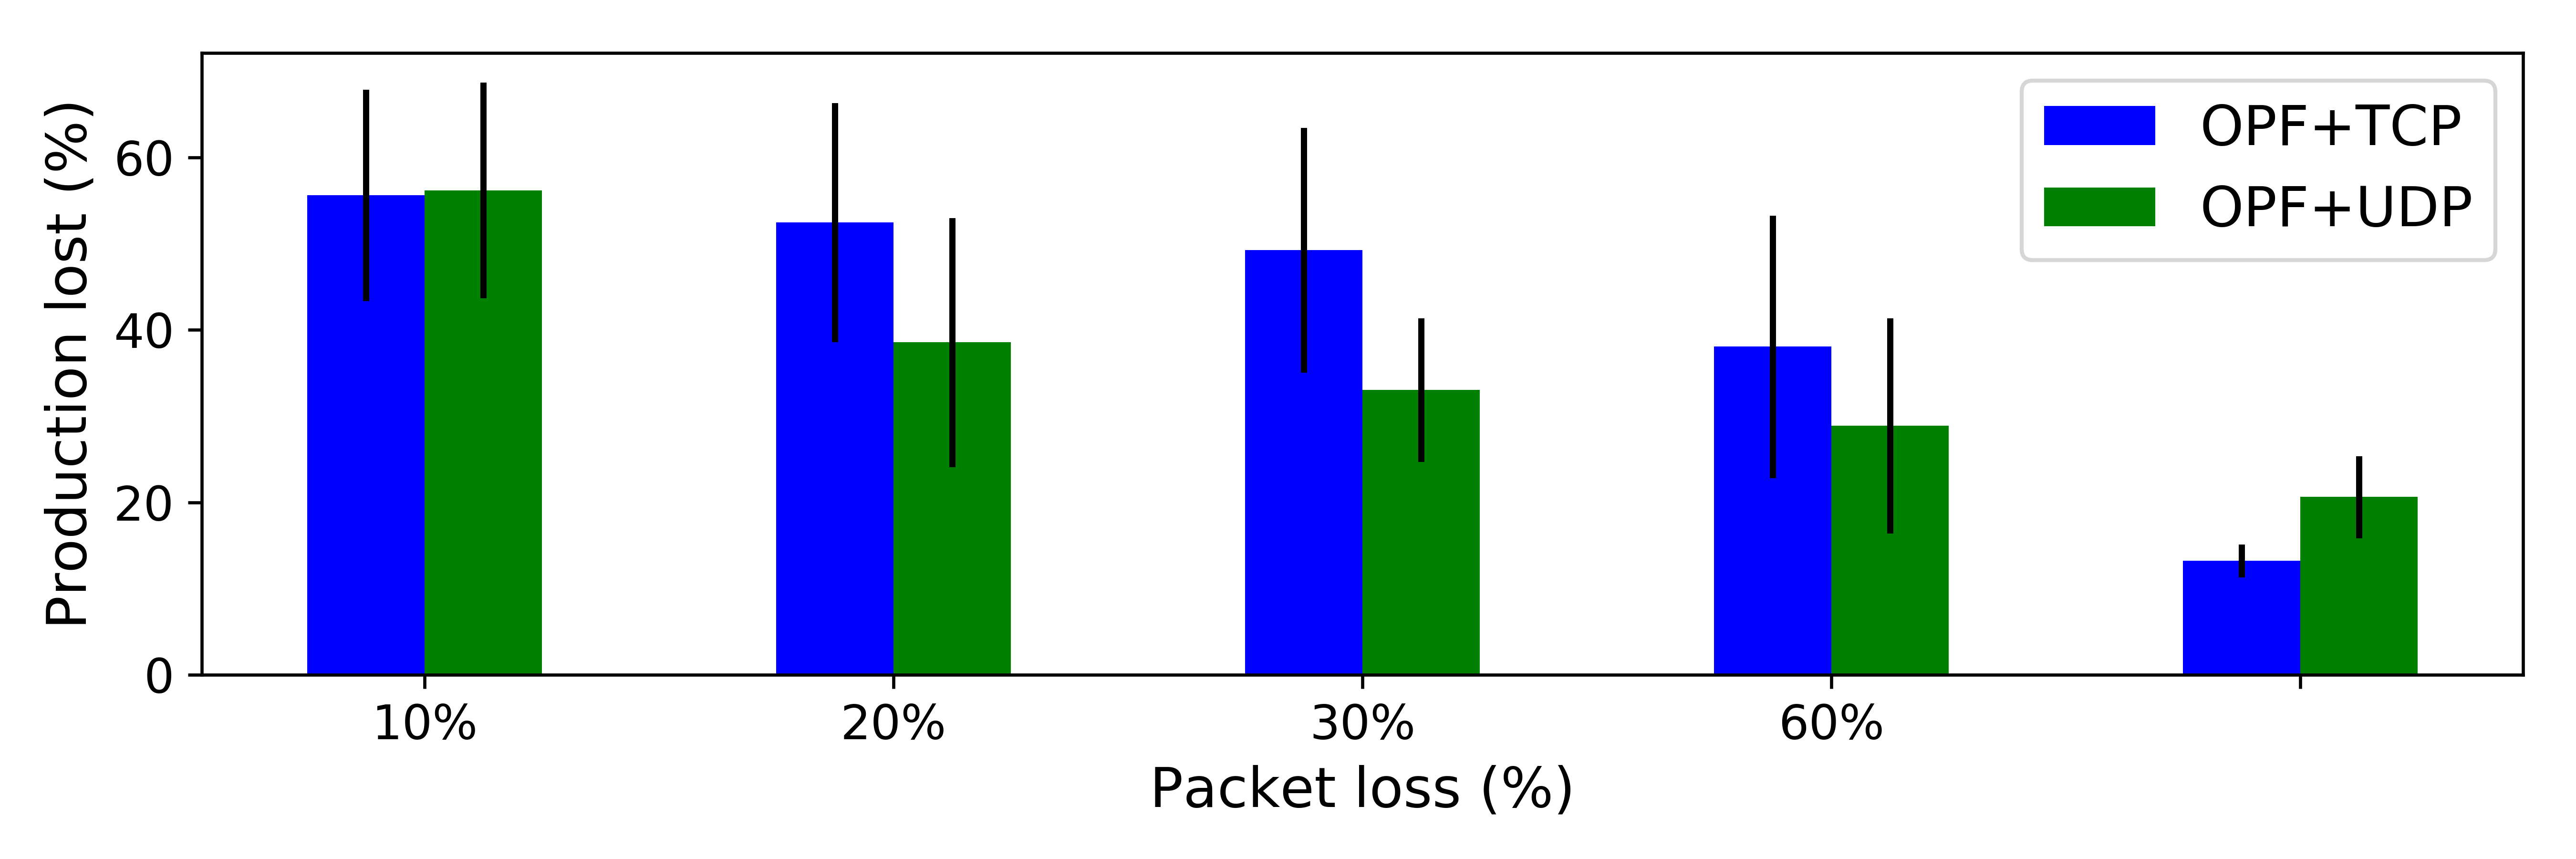
\includegraphics[width=0.5\textwidth]{bars_power_loss.png}
% 	\caption{Power production lost, with TCP/UDP communication on a lossy network}
% 	\label{bars_power_loss}
% \end{figure}

\section{Conclusion}
We have presented in this work, ASGriDS, a framework for the design, prototyping and testing of Smart Grid deployment scenarios through distributed and scalable simulation. In ASGrIDS, real-time control strategies can be implemented, and deployed on a communication network. ASGriDS allows the integration of emulated communication links, and/or the deployment over a physical ICT infrastructure. It provides a consistent workflow for describing complex multi-domain Smart Grid deployment scenarios. It is scalable and flexible, through a modular and asynchronous design. ASGriDS permits the various simulated components to exhibit behavior at various level of accuracy and complexity, and allows the integration of simulated power-network components, and the deployment of control strategies on physical communication hardware, or in combination with other hardware and software network components. A typical use-case is demonstrated, analyzing control performance over a lossy link, with two modes of communication, TCP and UDP.
ASGriDS is publicly available on a github repository\cite{TakiennAsgrids} together with the results described in this paper. We plan to continue its development, especially in distributed setups, with real ICT infrastructure and in HIL configurations. In this paper, we illustrated the capabilities of ASGriDS with a simple OPF controller described in~\eqref{eq_opf_1}. For future work, we plan to use ASGriDS to develop controllers that are fault tolerant and that can deal with measurement uncertainty and non-ideal communication.

\bibliographystyle{IEEEtran}  
\bibliography{lib}

\end{document}
